\hypertarget{_integral_invariant_8c}{
\section{/home/mgh/LanlGeoMag/libLanlGeoMag/IntegralInvariant.c File Reference}
\label{_integral_invariant_8c}\index{/home/mgh/LanlGeoMag/libLanlGeoMag/IntegralInvariant.c@{/home/mgh/LanlGeoMag/libLanlGeoMag/IntegralInvariant.c}}
}
{\tt \#include \char`\"{}Lgm/Lgm\_\-MagModelInfo.h\char`\"{}}\par


Include dependency graph for IntegralInvariant.c:\nopagebreak
\begin{figure}[H]
\begin{center}
\leavevmode
\includegraphics[width=291pt]{_integral_invariant_8c__incl}
\end{center}
\end{figure}
\subsection*{Defines}
\begin{CompactItemize}
\item 
\#define \hyperlink{_integral_invariant_8c_478cd83265b9c9a6b181dab783cb6fb8}{JUMP\_\-METHOD}~0
\item 
\#define \hyperlink{_integral_invariant_8c_77e2052ddd305972b5edf46998bde95b}{USE\_\-SIX\_\-POINT}~0
\item 
\#define \hyperlink{_integral_invariant_8c_9206839790faf94ac5c43e739b665505}{USE\_\-FOUR\_\-POINT}~1
\item 
\#define \hyperlink{_integral_invariant_8c_9b25b0c0eded8d7f0a08d985a2adb83c}{USE\_\-TWO\_\-POINT}~2
\item 
\#define \hyperlink{_integral_invariant_8c_c4ffbdb2f89837ddd347e7b6af16362f}{DIFF\_\-SCHEME}~USE\_\-TWO\_\-POINT
\end{CompactItemize}
\subsection*{Functions}
\begin{CompactItemize}
\item 
double \hyperlink{_integral_invariant_8c_f6e6b0cd75ad626d41e0ce06cbec7320}{Iinv} (\hyperlink{struct_lgm___mag_model_info}{Lgm\_\-MagModelInfo} $\ast$fInfo)
\item 
double \hyperlink{_integral_invariant_8c_ea31055ca3f80f4519c263c09ac3e832}{Iinv\_\-interped} (\hyperlink{struct_lgm___mag_model_info}{Lgm\_\-MagModelInfo} $\ast$fInfo)
\item 
double \hyperlink{_integral_invariant_8c_9a3dcc288db0c9c8153abd181494514e}{I\_\-integrand\_\-interped} (double s, \hyperlink{_lgm___quad_pack_8h_01be5a7db8d2fc2ba26ce793d73b6472}{\_\-qpInfo} $\ast$qpInfo)
\item 
double \hyperlink{_integral_invariant_8c_9378a29574f93271ed37929e9910f6c6}{I\_\-integrand} (double s, \hyperlink{_lgm___quad_pack_8h_01be5a7db8d2fc2ba26ce793d73b6472}{\_\-qpInfo} $\ast$qpInfo)
\item 
int \hyperlink{_integral_invariant_8c_daf0aa9fb80fcc0aa8addc079df7ac7c}{Grad\_\-I} (\hyperlink{struct_lgm___vector}{Lgm\_\-Vector} $\ast$v0, \hyperlink{struct_lgm___vector}{Lgm\_\-Vector} $\ast$GradI, \hyperlink{struct_lgm___mag_model_info}{Lgm\_\-MagModelInfo} $\ast$fInfo)
\end{CompactItemize}


\subsection{Define Documentation}
\hypertarget{_integral_invariant_8c_478cd83265b9c9a6b181dab783cb6fb8}{
\index{IntegralInvariant.c@{IntegralInvariant.c}!JUMP\_\-METHOD@{JUMP\_\-METHOD}}
\index{JUMP\_\-METHOD@{JUMP\_\-METHOD}!IntegralInvariant.c@{IntegralInvariant.c}}
\subsubsection[{JUMP\_\-METHOD}]{\setlength{\rightskip}{0pt plus 5cm}\#define JUMP\_\-METHOD~0}}
\label{_integral_invariant_8c_478cd83265b9c9a6b181dab783cb6fb8}




Definition at line 4 of file IntegralInvariant.c.\hypertarget{_integral_invariant_8c_77e2052ddd305972b5edf46998bde95b}{
\index{IntegralInvariant.c@{IntegralInvariant.c}!USE\_\-SIX\_\-POINT@{USE\_\-SIX\_\-POINT}}
\index{USE\_\-SIX\_\-POINT@{USE\_\-SIX\_\-POINT}!IntegralInvariant.c@{IntegralInvariant.c}}
\subsubsection[{USE\_\-SIX\_\-POINT}]{\setlength{\rightskip}{0pt plus 5cm}\#define USE\_\-SIX\_\-POINT~0}}
\label{_integral_invariant_8c_77e2052ddd305972b5edf46998bde95b}




Definition at line 6 of file IntegralInvariant.c.\hypertarget{_integral_invariant_8c_9206839790faf94ac5c43e739b665505}{
\index{IntegralInvariant.c@{IntegralInvariant.c}!USE\_\-FOUR\_\-POINT@{USE\_\-FOUR\_\-POINT}}
\index{USE\_\-FOUR\_\-POINT@{USE\_\-FOUR\_\-POINT}!IntegralInvariant.c@{IntegralInvariant.c}}
\subsubsection[{USE\_\-FOUR\_\-POINT}]{\setlength{\rightskip}{0pt plus 5cm}\#define USE\_\-FOUR\_\-POINT~1}}
\label{_integral_invariant_8c_9206839790faf94ac5c43e739b665505}




Definition at line 7 of file IntegralInvariant.c.\hypertarget{_integral_invariant_8c_9b25b0c0eded8d7f0a08d985a2adb83c}{
\index{IntegralInvariant.c@{IntegralInvariant.c}!USE\_\-TWO\_\-POINT@{USE\_\-TWO\_\-POINT}}
\index{USE\_\-TWO\_\-POINT@{USE\_\-TWO\_\-POINT}!IntegralInvariant.c@{IntegralInvariant.c}}
\subsubsection[{USE\_\-TWO\_\-POINT}]{\setlength{\rightskip}{0pt plus 5cm}\#define USE\_\-TWO\_\-POINT~2}}
\label{_integral_invariant_8c_9b25b0c0eded8d7f0a08d985a2adb83c}




Definition at line 8 of file IntegralInvariant.c.\hypertarget{_integral_invariant_8c_c4ffbdb2f89837ddd347e7b6af16362f}{
\index{IntegralInvariant.c@{IntegralInvariant.c}!DIFF\_\-SCHEME@{DIFF\_\-SCHEME}}
\index{DIFF\_\-SCHEME@{DIFF\_\-SCHEME}!IntegralInvariant.c@{IntegralInvariant.c}}
\subsubsection[{DIFF\_\-SCHEME}]{\setlength{\rightskip}{0pt plus 5cm}\#define DIFF\_\-SCHEME~USE\_\-TWO\_\-POINT}}
\label{_integral_invariant_8c_c4ffbdb2f89837ddd347e7b6af16362f}




Definition at line 10 of file IntegralInvariant.c.

\subsection{Function Documentation}
\hypertarget{_integral_invariant_8c_f6e6b0cd75ad626d41e0ce06cbec7320}{
\index{IntegralInvariant.c@{IntegralInvariant.c}!Iinv@{Iinv}}
\index{Iinv@{Iinv}!IntegralInvariant.c@{IntegralInvariant.c}}
\subsubsection[{Iinv}]{\setlength{\rightskip}{0pt plus 5cm}double Iinv ({\bf Lgm\_\-MagModelInfo} $\ast$ {\em fInfo})}}
\label{_integral_invariant_8c_f6e6b0cd75ad626d41e0ce06cbec7320}




Definition at line 42 of file IntegralInvariant.c.

Here is the call graph for this function:\nopagebreak
\begin{figure}[H]
\begin{center}
\leavevmode
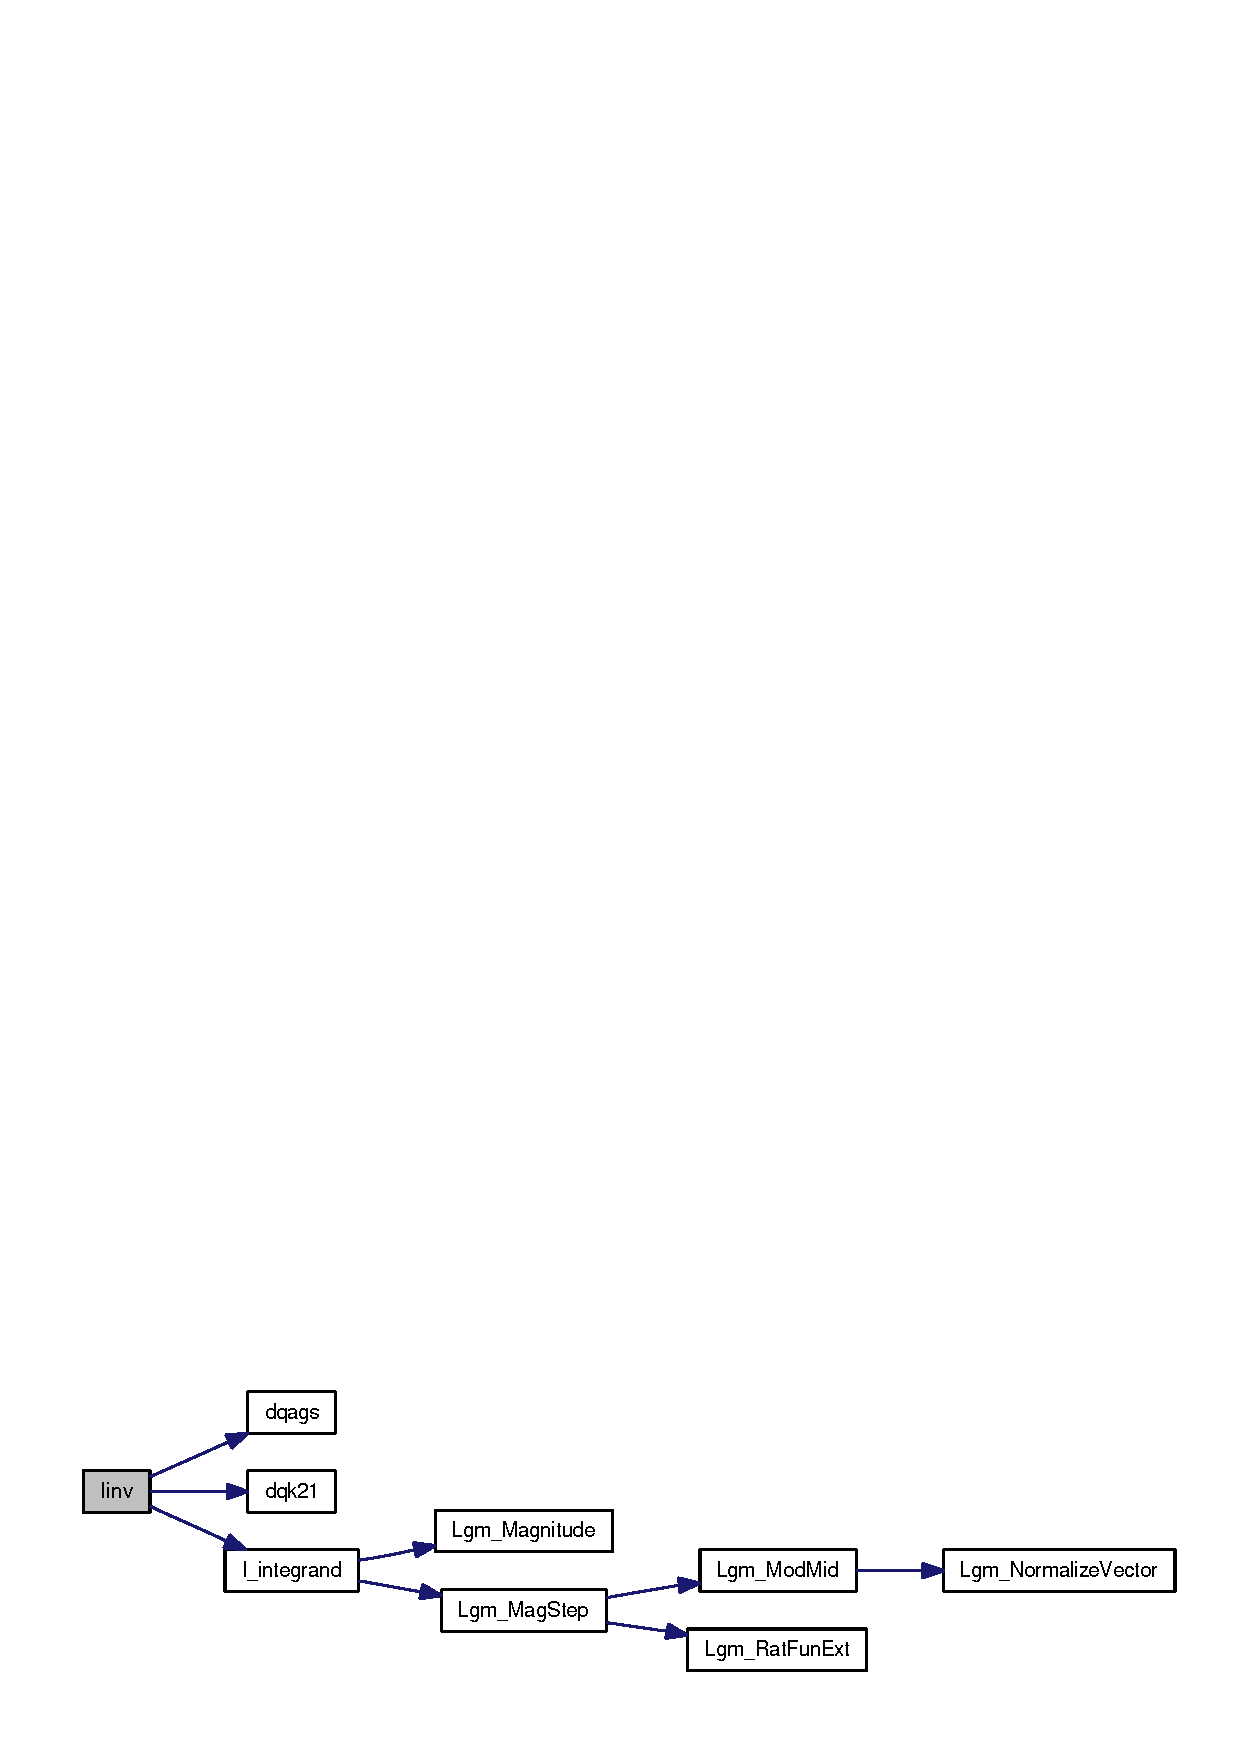
\includegraphics[width=284pt]{_integral_invariant_8c_f6e6b0cd75ad626d41e0ce06cbec7320_cgraph}
\end{center}
\end{figure}


Here is the caller graph for this function:\nopagebreak
\begin{figure}[H]
\begin{center}
\leavevmode
\includegraphics[width=141pt]{_integral_invariant_8c_f6e6b0cd75ad626d41e0ce06cbec7320_icgraph}
\end{center}
\end{figure}
\hypertarget{_integral_invariant_8c_ea31055ca3f80f4519c263c09ac3e832}{
\index{IntegralInvariant.c@{IntegralInvariant.c}!Iinv\_\-interped@{Iinv\_\-interped}}
\index{Iinv\_\-interped@{Iinv\_\-interped}!IntegralInvariant.c@{IntegralInvariant.c}}
\subsubsection[{Iinv\_\-interped}]{\setlength{\rightskip}{0pt plus 5cm}double Iinv\_\-interped ({\bf Lgm\_\-MagModelInfo} $\ast$ {\em fInfo})}}
\label{_integral_invariant_8c_ea31055ca3f80f4519c263c09ac3e832}




Definition at line 119 of file IntegralInvariant.c.

Here is the call graph for this function:\nopagebreak
\begin{figure}[H]
\begin{center}
\leavevmode
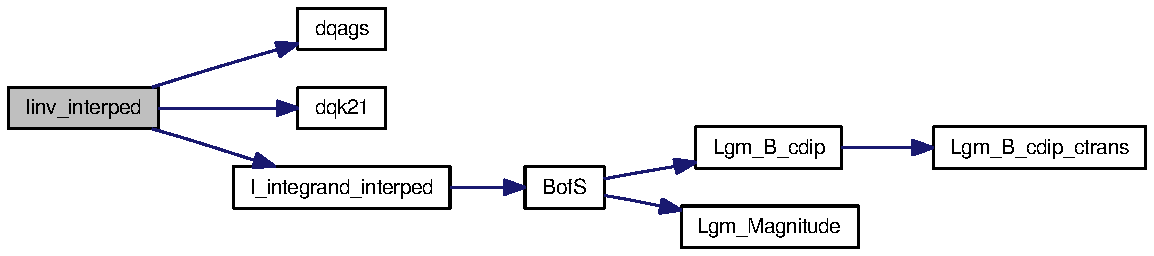
\includegraphics[width=295pt]{_integral_invariant_8c_ea31055ca3f80f4519c263c09ac3e832_cgraph}
\end{center}
\end{figure}


Here is the caller graph for this function:\nopagebreak
\begin{figure}[H]
\begin{center}
\leavevmode
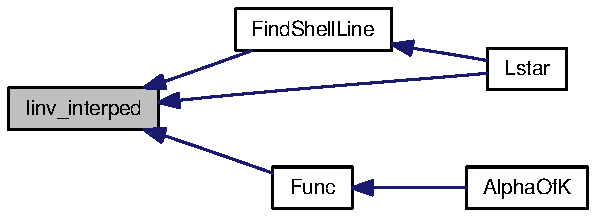
\includegraphics[width=161pt]{_integral_invariant_8c_ea31055ca3f80f4519c263c09ac3e832_icgraph}
\end{center}
\end{figure}
\hypertarget{_integral_invariant_8c_9a3dcc288db0c9c8153abd181494514e}{
\index{IntegralInvariant.c@{IntegralInvariant.c}!I\_\-integrand\_\-interped@{I\_\-integrand\_\-interped}}
\index{I\_\-integrand\_\-interped@{I\_\-integrand\_\-interped}!IntegralInvariant.c@{IntegralInvariant.c}}
\subsubsection[{I\_\-integrand\_\-interped}]{\setlength{\rightskip}{0pt plus 5cm}double I\_\-integrand\_\-interped (double {\em s}, \/  {\bf \_\-qpInfo} $\ast$ {\em qpInfo})}}
\label{_integral_invariant_8c_9a3dcc288db0c9c8153abd181494514e}




Definition at line 189 of file IntegralInvariant.c.

Here is the call graph for this function:\nopagebreak
\begin{figure}[H]
\begin{center}
\leavevmode
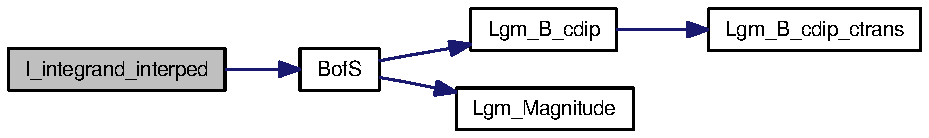
\includegraphics[width=241pt]{_integral_invariant_8c_9a3dcc288db0c9c8153abd181494514e_cgraph}
\end{center}
\end{figure}


Here is the caller graph for this function:\nopagebreak
\begin{figure}[H]
\begin{center}
\leavevmode
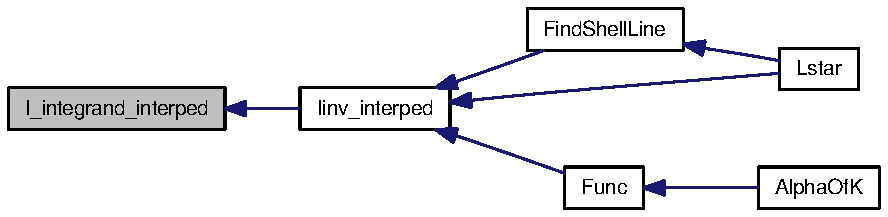
\includegraphics[width=231pt]{_integral_invariant_8c_9a3dcc288db0c9c8153abd181494514e_icgraph}
\end{center}
\end{figure}
\hypertarget{_integral_invariant_8c_9378a29574f93271ed37929e9910f6c6}{
\index{IntegralInvariant.c@{IntegralInvariant.c}!I\_\-integrand@{I\_\-integrand}}
\index{I\_\-integrand@{I\_\-integrand}!IntegralInvariant.c@{IntegralInvariant.c}}
\subsubsection[{I\_\-integrand}]{\setlength{\rightskip}{0pt plus 5cm}double I\_\-integrand (double {\em s}, \/  {\bf \_\-qpInfo} $\ast$ {\em qpInfo})}}
\label{_integral_invariant_8c_9378a29574f93271ed37929e9910f6c6}




Definition at line 217 of file IntegralInvariant.c.

Here is the call graph for this function:\nopagebreak
\begin{figure}[H]
\begin{center}
\leavevmode
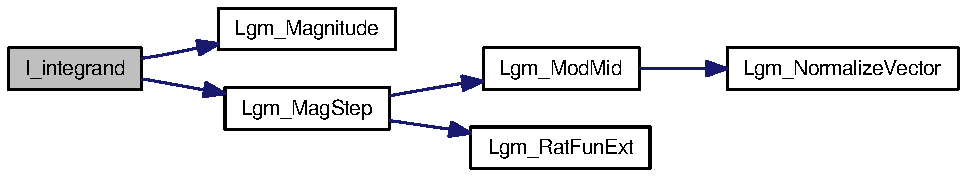
\includegraphics[width=250pt]{_integral_invariant_8c_9378a29574f93271ed37929e9910f6c6_cgraph}
\end{center}
\end{figure}


Here is the caller graph for this function:\nopagebreak
\begin{figure}[H]
\begin{center}
\leavevmode
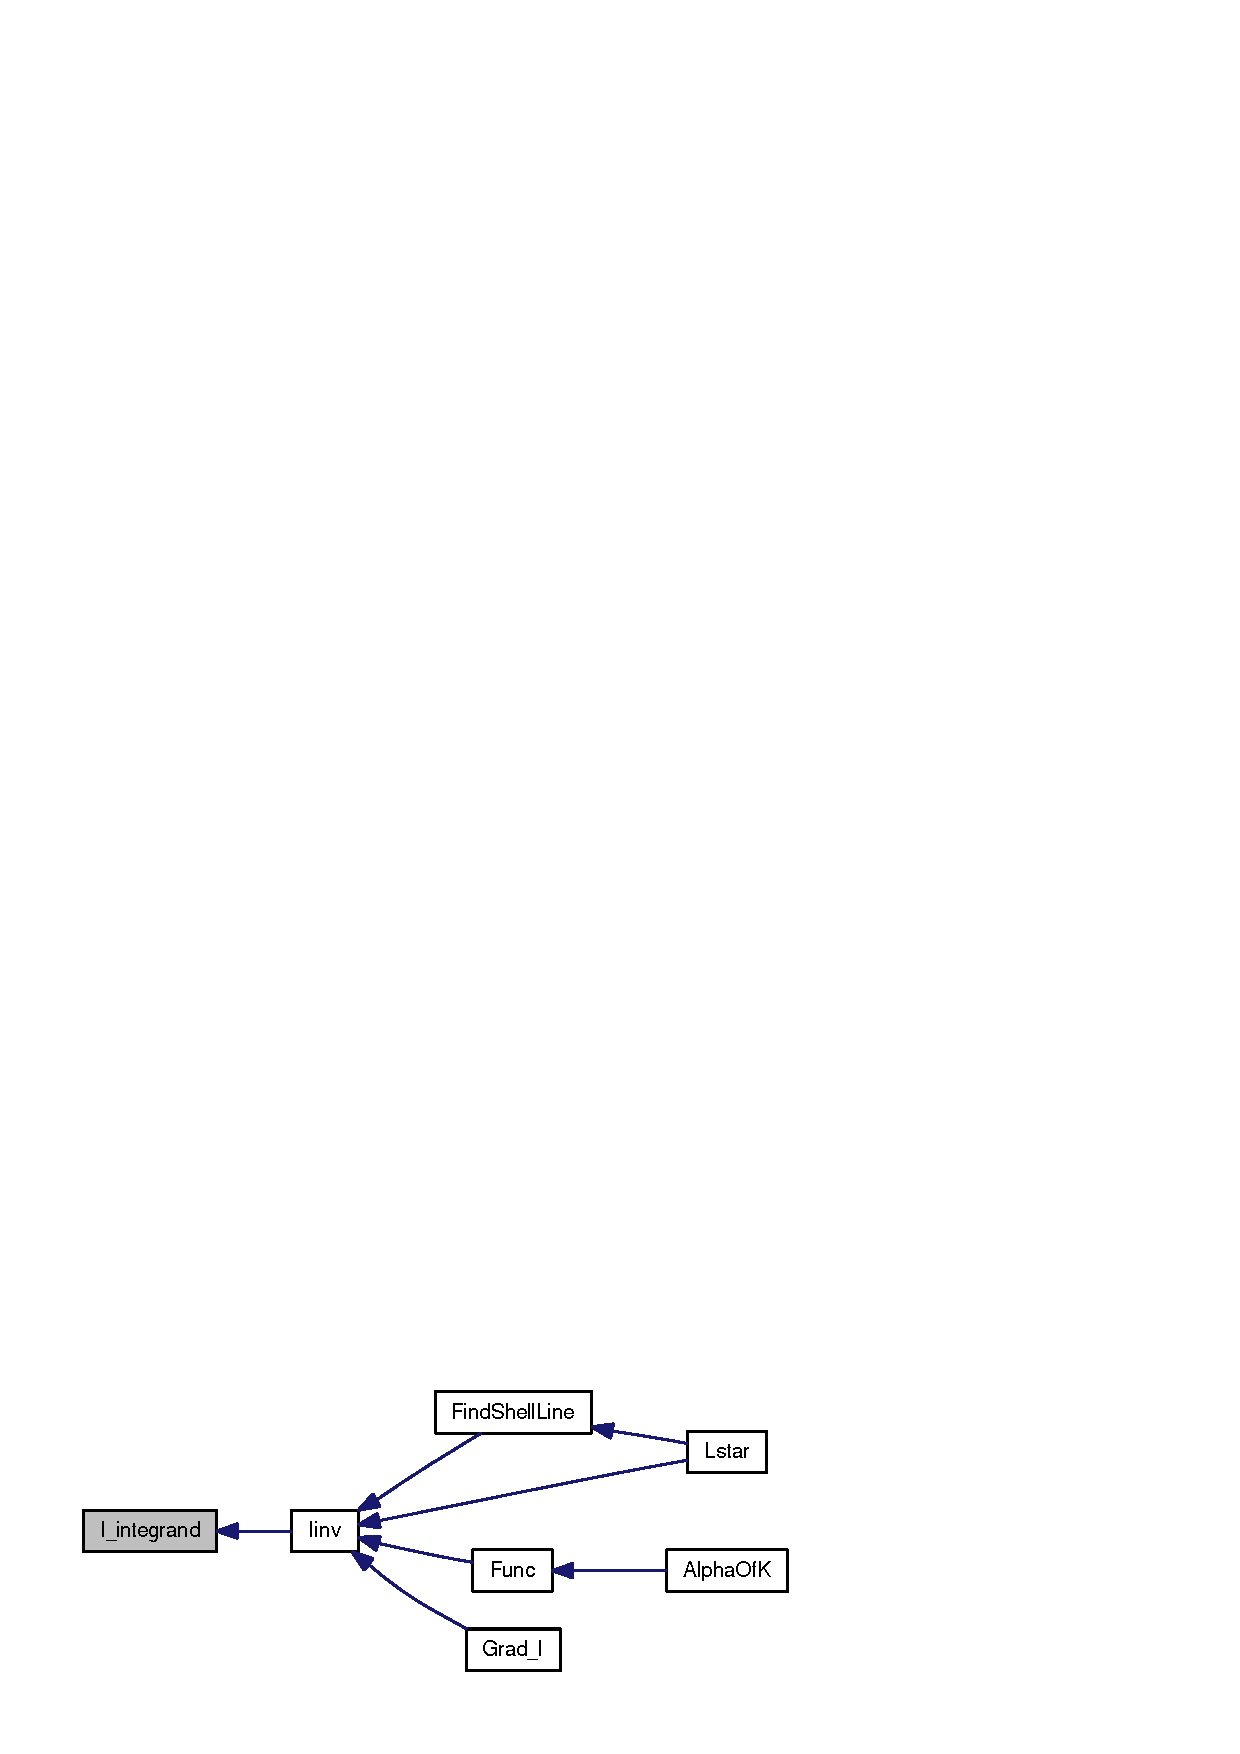
\includegraphics[width=191pt]{_integral_invariant_8c_9378a29574f93271ed37929e9910f6c6_icgraph}
\end{center}
\end{figure}
\hypertarget{_integral_invariant_8c_daf0aa9fb80fcc0aa8addc079df7ac7c}{
\index{IntegralInvariant.c@{IntegralInvariant.c}!Grad\_\-I@{Grad\_\-I}}
\index{Grad\_\-I@{Grad\_\-I}!IntegralInvariant.c@{IntegralInvariant.c}}
\subsubsection[{Grad\_\-I}]{\setlength{\rightskip}{0pt plus 5cm}int Grad\_\-I ({\bf Lgm\_\-Vector} $\ast$ {\em v0}, \/  {\bf Lgm\_\-Vector} $\ast$ {\em GradI}, \/  {\bf Lgm\_\-MagModelInfo} $\ast$ {\em fInfo})}}
\label{_integral_invariant_8c_daf0aa9fb80fcc0aa8addc079df7ac7c}




Definition at line 336 of file IntegralInvariant.c.

Here is the call graph for this function:\nopagebreak
\begin{figure}[H]
\begin{center}
\leavevmode
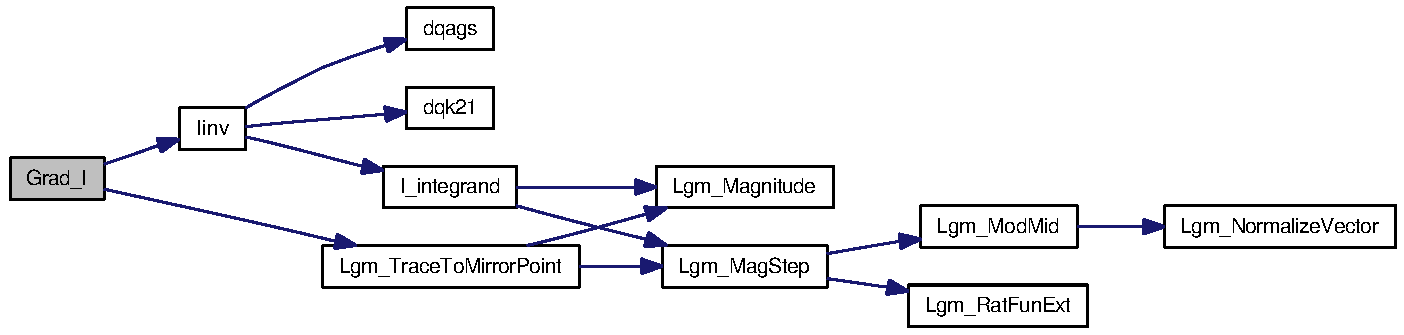
\includegraphics[width=355pt]{_integral_invariant_8c_daf0aa9fb80fcc0aa8addc079df7ac7c_cgraph}
\end{center}
\end{figure}
